\chapter{Introduction}
\label{ch:intro}

\begin{quote}
\textit{"So much of life, it seems to me, is determined by pure randomness"} –  Sidney Poitier	
\end{quote} 

As Sidney Poitier rightly stated, randomness determines many things in life, and so do random numbers.

In the modern era, random numbers play a significant role in many fields, including science, statistics, gaming, security, and many others, for various purposes \cite{RANDOM-1998}. For example, computer simulation and modelling of complex scenarios in artificial intelligence (AI) systems, where the scenarios are entirely unpredictable, the selection of random samples from enormous data sets for statistical analysis, data encryption, and games where indiscriminate numbers are instrumental, like an electronic casino and dice games \cite{RANDOM-1998} are just a few examples.

Speaking about other areas where random numbers are utilised, security and cryptography make great use of them. In cryptography, random numbers are used to create keys, salts, nonces, and other characteristics that make the protocols more unpredictable. Because of its unpredictable nature, it is challenging for an attacker to decrypt a communication without knowing the secret key that was used to encrypt it. It is necessary to utilise an excellent random number generator to guarantee the quality of randomness used in cryptographic protocols.


%
% Section: Need for Random Numbers in Embedded Environment
%
\section{Need for Random Numbers in the Embedded Environment}
\label{sec:intro:Need for Random Numbers in Embedded Environment}

The number of connected devices used today has increased, raising concerns about data privacy and unauthorised system access. Because embedded devices are a part of every connected device, their security is essential.

Another significant business adopting embedded devices in real-time embedded devices is the automotive industry. Tens to hundreds of electronic control units are present in every car on the road today, creating potential vulnerabilities for outsiders to enter, alter, and influence the vehicle’s behaviour. Further, changing the vehicle properties creates a severe safety concern. Hence, securing the device and every channel via which the communication to the vehicle is made is critical.

Considering the importance of random numbers in security from the previous part and the requirement for protecting embedded devices. The significant need for good random numbers in embedded devices can be explained.

%
% Section: Generation of Random Numbers
%
\section{Generation of Random Numbers}
\label{sec:intro:Generation of Random Numbers}

After discussing random numbers and their importance in the previous section, it is essential to understand how random numbers are generated and the possibility of generation in a closed embedded system.\\
Two approaches are available to generate the random numbers:

\begin{itemize}
	\item First approach is based on the physical process: This technique produces entirely non-deterministic random numbers. As the gathering process relies solely on physical phenomena such as weather and ring oscillators resulting in unexpected numbers, this type of generator is known as a non-deterministic random number generator (NRNG) or non-deterministic random bit generator (NRBG). Random number generators that produce such numbers are also known as true random number generators (TRNG) \cite{RANDOM-1998}.
	
	\item Second approach is based on a deterministic algorithm: This technique uses random numbers produced by several well-known public algorithms. Although the generated numbers appear random, they are not entirely random since the algorithm controls everything. As a result, they are often referred to as pseudo-random number generators (PRNG) that generate a sequence which repeats. This kind of generator is also known as a deterministic random number generator (DRNG) or deterministic random bit generator (DRBG) \cite{RANDOM-1998}.
\end{itemize}

Not all PRNGs, such as linear feedback shift registers (LFSR), can provide random numbers needed for security applications because cryptography demands highly reliable random numbers. Therefore, other PRNGs are permitted for use in cryptography called Cryptographically Secure Pseudo Random Number Generators (CSPRNG).

%
% Section: Motivation
%
\section{Motivation}
\label{sec:intro:structure}

NRBGs are ideally suited for cryptography since they create the most unexpected random numbers. Nevertheless, not all systems have TRNGs, and it takes a long time to generate random numbers using TRNGs.

In systems without TRNG, DRBG is necessary since it generates random numbers more quickly and on demand. However, deterministically produced numbers may be predicted. So, to make the random numbers unpredictable, we require input to the DRBG. Seed is the name given to such input, which will be discussed in chapter \ref{ch:fundamentals}. Random number unpredictability is solely dependent on the seed.
Thus, the seed’s durability is essential.

TRNGs are a fantastic seed source, but as already said, not all systems can support them. This highlights the need for a source that can provide random numbers to be utilised as a seed for DRBG. Entropy source is the name of this source. Entropy is a measure of a random number’s quality or unpredictability. Chapter \ref{ch:fundamentals} will comprehensively explain entropy, entropy source and available entropy sources.

The freshness values that the entropy source produces as an output make up most bits in the seed for the DRBG. Nevertheless, using real-time embedded devices has significant disadvantages that make obtaining the necessary entropy more challenging.

The following are the fundamental causes of difficulties in extracting sufficient entropy in embedded real-time systems, such as electronic control units (ECU) in the automobile domain:

\begin{itemize}
	\item To determine if enough entropy has been acquired, the amount of entropy produced by the source in one sample is unknown.
	\item The absence of sources that are typically accessible in most of the ECUs.
	\item If any source is available primarily in all ECU, such sources may not produce the same amount of entropy in every ECU.	
	\item The amount of entropy accessible at start-up is insufficient due to the shorter boot time.	
	\item The absence of often changing user human interfaces, such as keystrokes.	
	\item Using predefined seeds during every active cycle of ECU is often ineffective since they might be compromised. 
\end{itemize}

The general idea of cyber security may deteriorate with insufficient entropy \cite{SP90B-2018}. As shown in figure \ref{fig:1:1}, although the notion of cybersecurity is quite solid, if sufficient entropy is not given, it is equivalent to building a massive structure on unstable ground. We are never sure when a structure will crumble.

\begin{figure}[!h]
	\centering
	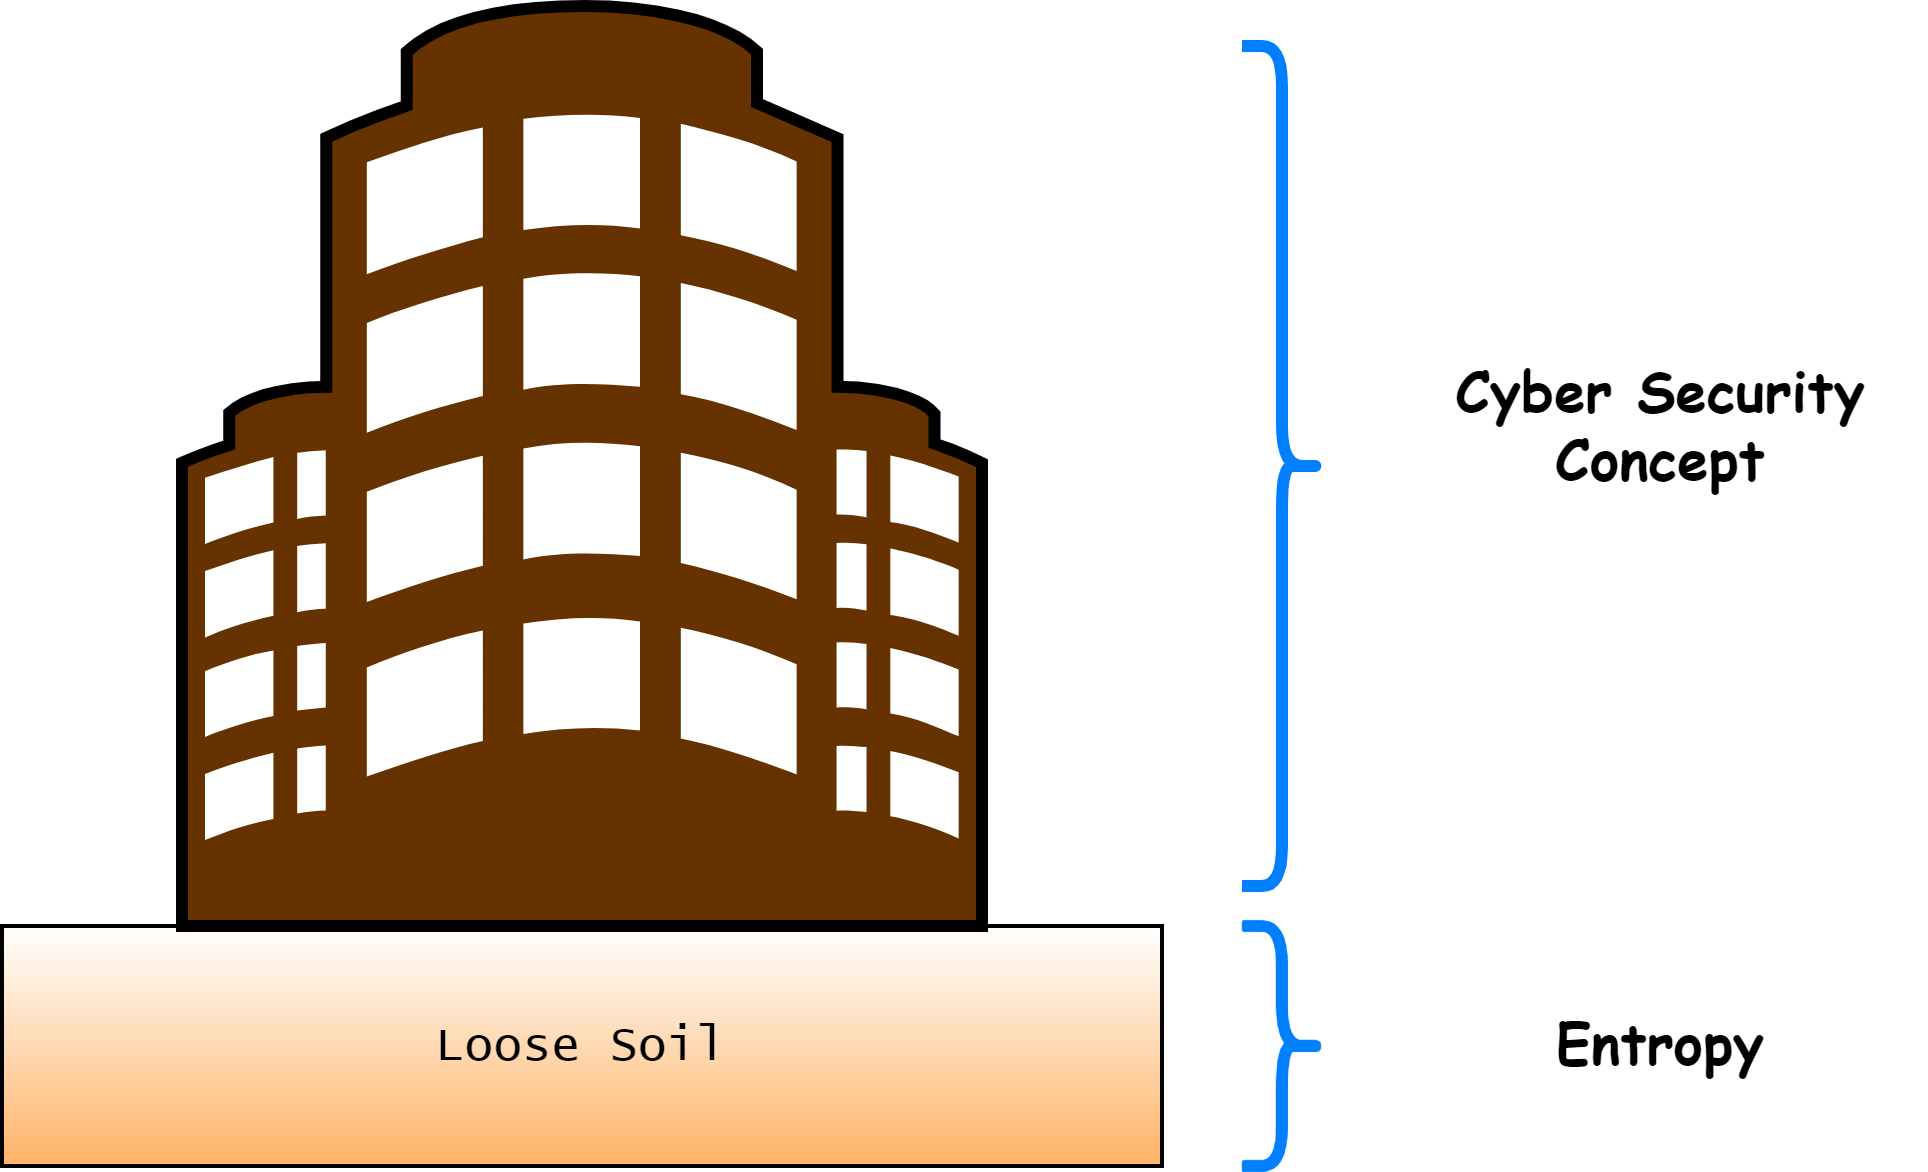
\includegraphics[width=0.75\textwidth]{gfx/diagrams/EffectOfWeakEntropy}
	\caption{Illustration of dependency of security concept on entropy}
	\label{fig:1:1}
\end{figure}

The fact that entropy is a fundamental component of cryptography/security motivates us to understand more about available entropy sources and ways to enhance the reliability of random numbers in ECU. Chapter \ref{ch:CD} provides a comprehensive discussion of the limitations, as mentioned earlier.

%
% Section: Objective
%
\section{Objective}
\label{sec:intro:Objective}

As seen in the preceding section, we need a universal remedy that works in most ECUs without TRNG to reduce the frequent problems. The purpose of this thesis is to locate and evaluate potential sources of entropy within the ECU to generate a sufficiently good (to satisfy security needs) seed, comprehend the requirements from the NIST SP 800-90 standard series (National Institute of Standards and Technology - Special Publication), and design an architecture that aids in gathering enough entropy from sources for the system to be secure. Furthermore, to manage the boot time entropy requirement.

Furthermore, a UI-based (user interface) Framework must be designed and developed to automatically produce code following the proposed architecture based on NIST standards. Framework avoids the hurdle for developers to implement entirely in every project requiring such architecture. This Framework also provides an interface to support any source. The Framework should be able to record the following user inputs:

\begin{itemize}
	\item Required security strength.
	\item Selection of entropy sources.
	\item Scheduling entropy collection from sources.
	\item Runtime validation of the entropy sources.
\end{itemize}

The Framework’s ability to produce code ready for integration based on user inputs should be evaluated and confirmed. The final product of the created code should behave like a TRNG and provide high-quality random numbers that can be seeded into DRBG to produce the random numbers.

The entropy source’s operational circumstances and attack vectors must be determined. Subsequently, techniques must be created to mitigate circumstances under which random numbers are compromised for any cause, weakening security.

To achieve the objective described earlier, available state-of-the-art (SoA) was analysed, which is described in detail in chapter \ref{ch:SoA}. Practical limitations to achieving the goal using SoA were weighed. Considering every factor that impacts the target, an architecture was designed.

Intermittent goals for achieving the final objective of improving the quality of random numbers for use in automotive ECUs can be summarised as follows:
\begin{itemize}
	\item Identification of potential noise sources.
	\item Design and implement an architecture to collect entropy from the source and improve the seed to satisfy entropy requirements during boot and runtime.
	\item Framework design to ease the implementation for developers.
\end{itemize}

%
% Section: Thesis Outline
%
\section{Thesis Outline}
\label{sec:intro:Thesis Outline}

The following sentences provide a summary of this thesis and its organisation before getting into further detail:

\begin{description}
	\item[Chapter \ref{ch:fundamentals} (Fundamentals)] The essentials, including entropy, different forms of entropy, and other terminology, are covered in this chapter.
	
	\item[Chapter \ref{ch:SoA} (State of the Art)] Here, we try comprehending earlier studies on a related subject. Explain the pooling algorithms that the standard recommends for embedded systems, including Fortuna and Linux RNG.
	
	\item[Chapter \ref{ch:CD} (Conceptual Design)] In this chapter, we detail the issue statement and outline the requirements based on it and the elements of the problem statement that cannot be handled using the state-of-the-art (SoA). An explanation of the concept’s architecture, a justification of how the idea solves the issue indicated in the reason. Provide a design for Framework.
	
	\item[Chapter \ref{ch:Imp} (Implementation)] The implementation of the notion discussed in chapter \ref{ch:CD} is described in this chapter, explaining each component of the Framework, how it was used, and how to incorporate it into current applications.
	
	\item[Chapter \ref{ch:RA} (Results and Analysis)] This chapter analyses the architectural design theoretically, outlining its benefits and shortcomings. Furthermore, it evaluates the target entropy’s risk.
	
	\item[Chapter \ref{ch:end} (Outline and conclusion)] This chapter concludes the thesis with recommendations and future work that can/needs to be done.
\end{description}


